\documentclass{standalone}
\usepackage{graphicx}	
\usepackage{amssymb, amsmath, amsthm}
\usepackage{color}

\usepackage{tikz}
\usetikzlibrary{math, calc}

\definecolor{light}{RGB}{220, 188, 188}
\definecolor{mid}{RGB}{185, 124, 124}
\definecolor{dark}{RGB}{143, 39, 39}
\definecolor{highlight}{RGB}{180, 31, 180}
\definecolor{gray10}{gray}{0.1}
\definecolor{gray20}{gray}{0.2}
\definecolor{gray30}{gray}{0.3}
\definecolor{gray40}{gray}{0.4}
\definecolor{gray60}{gray}{0.6}
\definecolor{gray70}{gray}{0.7}
\definecolor{gray80}{gray}{0.8}
\definecolor{gray90}{gray}{0.9}
\definecolor{gray95}{gray}{0.95}
  
\newcommand{\drawcube}[4]{
  \pgfmathsetmacro{\dx}{#1}
  \pgfmathsetmacro{\dy}{#2} 
  \pgfmathsetmacro{\dz}{#3}  
  \pgfmathsetmacro{\tilt}{#4}
  
  \fill[light]    ({-(1 - \tilt) * \dx}, -\dy + \dz) 
               -- ({(1 + \tilt) * \dx}, -\dy + \dz) 
               -- ({(1 - \tilt) * \dx}, \dy + \dz) 
               -- ({-(1 + \tilt) * \dx}, \dy + \dz) -- cycle;  

  \fill[mid]    ({-(1 - \tilt) * \dx}, -\dy) 
             -- ({-(1 - \tilt) * \dx}, -\dy + \dz)
             -- ({-(1 + \tilt) * \dx}, \dy + \dz) 
						 -- ({-(1 + \tilt) * \dx}, \dy) -- cycle;

  \fill[dark]    ({-(1 - \tilt) * \dx}, -\dy) 
              -- ({(1 + \tilt) * \dx}, -\dy)
              -- ({(1 + \tilt) * \dx}, -\dy + \dz) 
              -- ({-(1 - \tilt) * \dx}, -\dy + \dz) -- cycle;
                       
  \draw[dark]    ({(1 + \tilt) * \dx}, -\dy) 
              -- ({(1 + \tilt) * \dx}, -\dy + \dz) 
              -- ({(1 - \tilt) * \dx}, \dy + \dz) 
              -- ({-(1 + \tilt) * \dx}, \dy + \dz)
              -- ({-(1 + \tilt) * \dx}, \dy) 
              -- ({-(1 - \tilt) * \dx}, -\dy)
              -- cycle;
              
 \draw[dark]    ({-(1 + \tilt) * \dx + 0.01}, \dy + \dz) 
             -- ({-(1 - \tilt) * \dx + 0.01}, -\dy + \dz) 
             -- ({(1 + \tilt) * \dx + 0.01}, -\dy + \dz);
}

\newcommand{\drawcubecageback}[4]{
  \pgfmathsetmacro{\dx}{#1}
  \pgfmathsetmacro{\dy}{#2} 
  \pgfmathsetmacro{\dz}{#3}  
  \pgfmathsetmacro{\tilt}{#4}
                   
  \draw[dark, dashed]    ({(1 - \tilt) * \dx}, \dy) 
                      -- ({(1 - \tilt) * \dx}, \dy + \dz) 
                      -- ({-(1 + \tilt) * \dx}, \dy + \dz) 
                      -- ({-(1 + \tilt) * \dx}, \dy) 
                      -- cycle;
}

\newcommand{\drawcubecagefront}[4]{
  \pgfmathsetmacro{\dx}{#1}
  \pgfmathsetmacro{\dy}{#2} 
  \pgfmathsetmacro{\dz}{#3}  
  \pgfmathsetmacro{\tilt}{#4}
                   
  \draw[dark, dashed]    ({(1 + \tilt) * \dx}, -\dy) 
                      -- ({(1 + \tilt) * \dx}, -\dy + \dz) 
                      -- ({-(1 - \tilt) * \dx + 0.015}, -\dy + \dz) 
                      -- ({-(1 - \tilt) * \dx + 0.015}, -\dy) 
                      -- cycle;
                      
  \draw[dark, dashed]    ({-(1 + \tilt) * \dx + 0.01}, \dy + \dz) 
                      -- ({-(1 - \tilt) * \dx + 0.01}, -\dy + \dz);

  \draw[dark, dashed]    ({(1 - \tilt) * \dx}, \dy + \dz) 
                      -- ({(1 + \tilt) * \dx}, -\dy + \dz);
             
}

\begin{document}

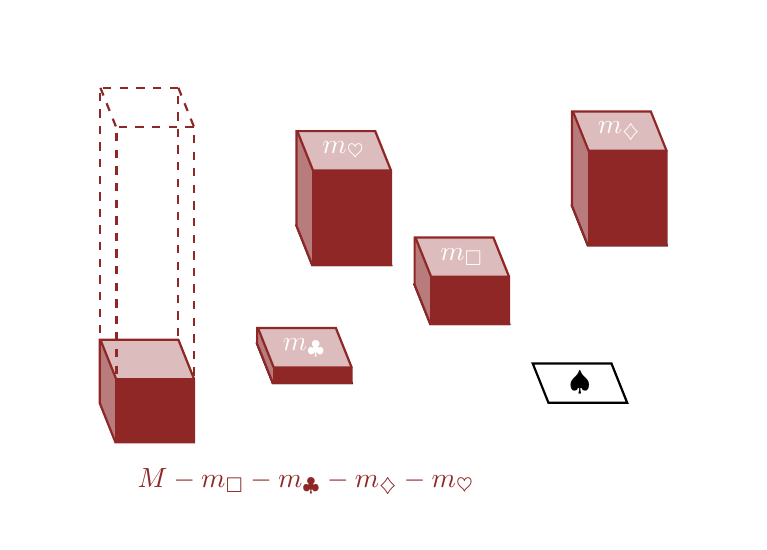
\begin{tikzpicture}[scale=1, thick]

  \draw[white] (-5.5, -2.75) rectangle (3.5, 3.5);
  
  \pgfmathsetmacro{\dx}{0.5}
  \pgfmathsetmacro{\dy}{0.25}
  \pgfmathsetmacro{\dz}{1}
  \pgfmathsetmacro{\tilt}{0.2}
  
  \foreach \x/\y\glyph [count=\n] in {0/0/\Box, -2/-0.75/\clubsuit, 2/1/\diamondsuit, 
                                      -1.5/0.75/\heartsuit, 1.5/-1/\spadesuit} {
    \begin{scope}[shift={(\x, \y)}]
      \node at (0, 0) { $\glyph$ };
      \draw[black]    ({-(1 - \tilt) * \dx}, -\dy) -- ({(1 + \tilt) * \dx}, -\dy) 
                   -- ({(1 - \tilt) * \dx}, \dy) -- ({-(1 + \tilt) * \dx}, \dy) -- cycle;
    \end{scope}
  }

  \foreach \x/\y/\p/\glyph [count=\n] in {0/0/0.15/\Box, -2/-0.75/0.05/\clubsuit, 2/1/0.3/\diamondsuit, -1.5/0.75/0.3/\heartsuit} {
    \begin{scope}[shift={(\x, \y)}]
      \drawcube{\dx}{\dy}{4 * \p}{\tilt}
      \node[white] at (0, {4 * \p}) { $m_{\glyph}$ };
    \end{scope}
  }

  \begin{scope}[shift={(-4, -1.5)}]
    \drawcubecageback{\dx}{\dy}{4}{\tilt}
    \drawcube{\dx}{\dy}{4 * (1 - 0.8)}{\tilt}
    \drawcubecagefront{\dx}{\dy}{4}{\tilt}
  \end{scope}
  
  \node[dark, anchor=west] at (-4.25, -2.25) { $M - m_\Box - m_\clubsuit - m_\diamondsuit - m_\heartsuit$ };

\end{tikzpicture}

\end{document}  